\documentclass[a4paper]{iacas}

\usepackage{cite}
\usepackage{hyperref}% embedding hyperlinks [must be loaded after dropping]
\usepackage{amsmath,amsthm,amssymb,amsfonts,latexsym,mathrsfs,wasysym}
\usepackage{marvosym}
\usepackage{subcaption}
\usepackage{soul,color}
\usepackage{threeparttable}% tables with footnotes
\usepackage{dcolumn}% decimal-aligned tabular math columns
\usepackage{float}
\usepackage{graphicx}
\usepackage{accents}
\usepackage{tikz}
\usepackage{lastpage}
\usepackage{fancyhdr}
\usepackage{color}
\usepackage{cancel}
\usepackage{setspace}
\usepackage{enumitem}

%\doublespacing
% or:
\onehalfspacing
%\usepackage[T1]{fontenc}
%\usepackage{bigfoot} % to allow verbatim in footnote
\usepackage[framed,numbered]{matlab-prettifier}
\pagestyle{plain}
%\usepackage[hebrew,english]{babel}
\usetikzlibrary{shapes.geometric, arrows, calc}

\newcolumntype{d}{D{.}{.}{-1}}
\graphicspath{{figures/}}

% define some commands to maintain consistency
\newcommand{\pkg}[1]{\texttt{#1}}
\newcommand{\cls}[1]{\textsf{#1}}
\newcommand{\file}[1]{\texttt{#1}}
\newcommand{\sgn}[1]{\operatorname{sgn}\left(#1\right)}
\newcommand{\sat}[1]{\operatorname{sat}\left(#1\right)}
\newcommand{\rrule}[1]{\rule[#1]{0pt}{0pt}}
\newcommand{\fracds}[2]{\frac{\displaystyle #1\rrule{-0.2em}}{\displaystyle #2\rrule{1em}}}
\newcommand{\figref}[1]{Fig.~\ref{#1}}
\newcommand{\ubar}[1]{\underaccent{\bar}{#1}}
\newcommand{\norm}[1]{\lvert \lvert \vec #1 \rvert \rvert}

%diffeomorphism

\begin{document}

\begin{center}
 \large Algorithms and Application in Computer Vision - 046746
 \end{center}
\begin{center}
\large\textbf{Homework \#2}
 \end{center}


\begin{tabular}{l}
\\
{\bf\textit{Alexander Shender 328626114}} \\
{\bf\textit{Vladimir Tchuiev 309206795}} \\
Technion - Israel Institute of Technology
\end{tabular}


\newpage

\section{Dry section}

\subsection{Question 1.}
\subsubsection{a.}

The dimensions of the layers change in the following way:
\newline
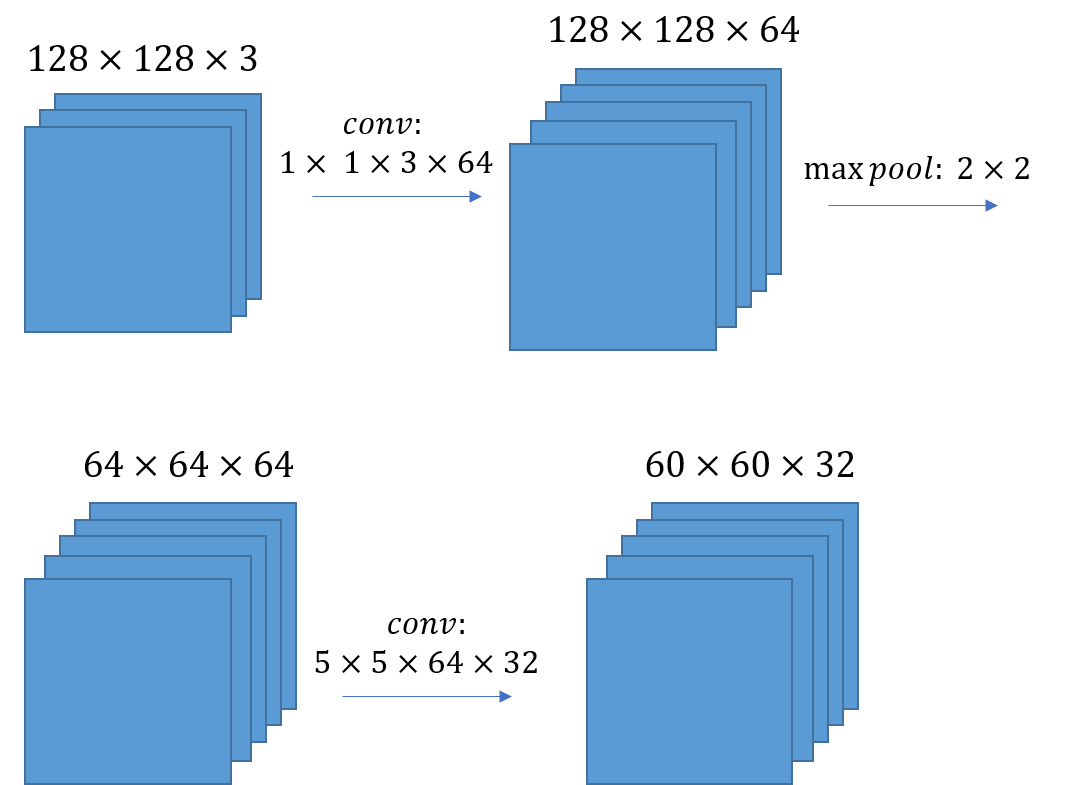
\includegraphics[scale=0.7]{imgs/q_1_1.png}
\newline
\subsubsection{b.}
The convolution of the size 1X1X(?) performs convolution on the same pixes in different channels. The input image contains 3 channels in our case, thus the convolution of the size 1X1X3 fits perfectly to result in a block of new layers without changing size (no need for padding). One kernel results in an output layer of size $128\times128$, but since we have 64 kernels, the depth of the next layers block is 64, accordingly.

\subsubsection{c.}
Let's say, our normalized filter is the following:
\begin{equation*}
\left[
\begin{matrix}
0.1 & 0.2 & 0. 05 \\
0.05 & 0.2 & 0.1 \\
0.15 & 0.1 & 0.05
\end{matrix}
\right]
\end{equation*}

We choose 2 options for stride and padding:

\begin{enumerate}
\item $stride = 2, padding = 1$
The image now has a dimensions of $9\times9$, and with a stride of 1 it gives an output dimensions: $3\times3$
\newline
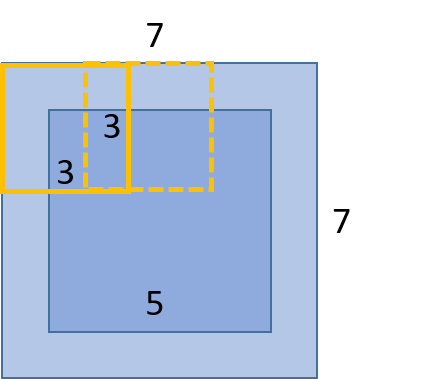
\includegraphics[scale=0.8]{imgs/q_1_31.png}
\newline
Output result is the following:

\begin{equation*}
\left[
\begin{matrix}
1.3 & 2.7 & 1.9 \\
1.9 & 5.25 & 3.1 \\
0.5 & 3.5 & 1.7
\end{matrix}
\right]
\end{equation*}


\item $stride = 1, padding = 2$
The image now has a dimensions of $7\times7$, but with stride of 2 it fits with the filter. Output dimensions: $7\times7$
\newline
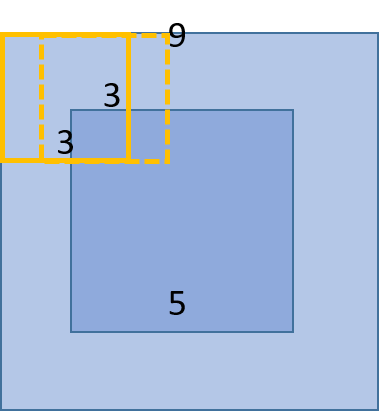
\includegraphics[scale=0.8]{imgs/q_1_32.png}
\newline
Output result is the following:

\begin{equation*}
\left[
\begin{matrix}
0.2 & 0.45 & 1 & 0.8 & 1.15 & 0.45 & 0.45 \\
0.55 & 1.3 & 2.0 & 2.7 & 2.65 & 1.9 & 0.45 \\
0.6 & 2.1 & 3.3 & 5.15 & 4.6 & 2.6 & 1.45\\
0.4 & 1.9 & 3.75 & 5.25 & 5.145 & 3.1 & 1 \\
0.2 & 1.3 & 3.5 & 4.7 & 4.0 & 3.35 & 1.45\\
0.05 & 0.5 & 2.05 & 3.5 & 2.55 & 1.7 & 0.5 \\ 
0 & 0.05 & 0.5 & 1.5 & 1.6 & 1.2 & 0.4
\end{matrix}
\right]
\end{equation*}
\end{enumerate}.
The code is provided in the appendix.


\newpage
\subsection{Question 2.}
The architecture selected is the VGG16 architecture. The image found in the internet which describes the structure is the following:
\newline
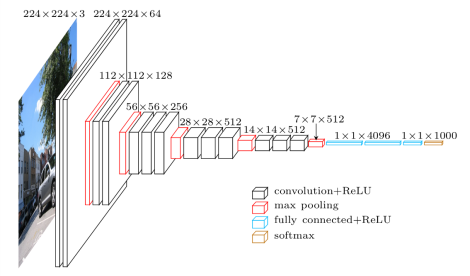
\includegraphics[scale=0.6]{imgs/vgg_arc.PNG}
\newline

Writing the exact outputs for every layer:

\begin{table}[]
\begin{tabular}{|l|l|l|l|l|l}
\cline{1-5}
Operation       & Size                   & Padding   & Stride & Output size       &  \\ \cline{1-5}
Conv block      & {[}3X3X3{]}X64         & {[}1 1{]} & 1      & {[}224X224X64{]}  &  \\ \cline{1-5}
Conv block      & {[}3X3X64{]}X64        & {[}1 1{]} & 1      & {[}224X224X64{]}  &  \\ \cline{1-5}
Pool 2D         & {[}2 2{]}              & N/A       & N/A    & {[}112X112X64{]}  &  \\ \cline{1-5}
Conv block      & {[}3X3X64{]}X128       & {[}1 1{]} & 1      & {[}112X112X128{]} &  \\ \cline{1-5}
Conv block      & {[}3X3X128{]}X128      & {[}1 1{]} & 1      & {[}112X112X128{]} &  \\ \cline{1-5}
Pool 2D         & {[}2 2{]}              & N/A       & N/A    & 56X56X128         &  \\ \cline{1-5}
Conv block      & {[}3X3X128{]}X256      & {[}1 1{]} & 1      & {[}56X56X256{]}   &  \\ \cline{1-5}
Conv block      & {[}3X3X256{]}X256      & {[}1 1{]} & 1      & {[}56X56X256{]}   &  \\ \cline{1-5}
Conv block      & {[}3X3X256{]}X256      & {[}1 1{]} & 1      & {[}56X56X256{]}   &  \\ \cline{1-5}
Pool 2D         & {[}2 2{]}              & N/A       & N/A    & {[}28X28X256{]}   &  \\ \cline{1-5}
Conv block      & {[}3X3X256{]}X512      & {[}2 2{]} & 1      & {[}28X28X512{]}   &  \\ \cline{1-5}
Conv block      & {[}3X3X512{]}X512      & {[}2 2{]} & 1      & {[}28X28X512{]}   &  \\ \cline{1-5}
Conv block      & {[}3X3X512{]}X512      & {[}2 2{]} & 1      & {[}28X28X512{]}   &  \\ \cline{1-5}
Pool 2D         & {[}2 2{]}              & N/A       & N/A    & {[}14X14X512{]}   &  \\ \cline{1-5}
Conv block      & {[}3X3X512{]}X512      & {[}1 1{]} & 1      & {[}14X14X512{]}   &  \\ \cline{1-5}
Conv block      & {[}3X3X512{]}X512      & {[}1 1{]} & 1      & {[}14X14X512{]}   &  \\ \cline{1-5}
Conv block      & {[}3X3X512{]}X512      & {[}1 1{]} & 1      & {[}14X14X512{]}   &  \\ \cline{1-5}
Conv block      & {[}3X3X512{]}X512      & {[}1 1{]} & 1      & {[}14X14X512{]}   &  \\ \cline{1-5}
Pool 2D         & {[}2 2{]}              & N/A       & N/A    & {[}7X7X512{]}     &  \\ \cline{1-5}
Fully connected & {[}7$\cdot$7$\cdot$512{]}X4096 & N/A       & N/A    & {[}1X1X4096{]}    &  \\ \cline{1-5}
Fully connected & {[}4096X4096{]}        & N/A       & N/A    & {[}1X1X4096{]}    &  \\ \cline{1-5}
Fully connected & {[}4096X1000{]}        & N/A       & N/A    & {[}1X1X1000{]}    &  \\ \cline{1-5}
\end{tabular}
\end{table}

\newpage
\subsection{Question 3.}
\textbf{Definition: }Overfitting - is a situation, where network is fitted too much to the training data, and finds it difficult to generalize to create predictions for the new data. 
\newline
\textbf{How to spot: }First of all, a researcher will notice that the accuracy of the model on the Test Dataset decreases, while the accuracy on the Training Set will still be increasing. The typical graph vizuasing error on the Test \& Training set may be seen, demonstrating this exact situation:
\newline
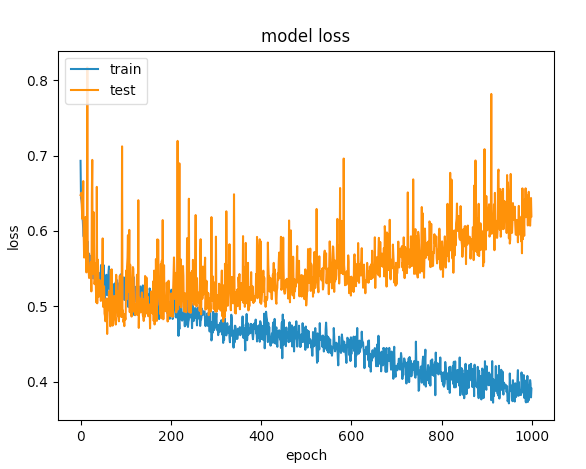
\includegraphics[scale=0.4]{imgs/overfit.PNG}
\newline
\textbf{How to avoid: }There are numerous way to avoid overfitting:
\begin{enumerate}
\item Stop the training before the accuracy for the validation set starts increasing. If the accuracy does not satisfy, find a better dataset / improve the network / apply other changes. Training for more time will worsen the situation.
\item Use one of the following methods: regularisation, lambda factor, dropout, etc.
\item Increase the dataset size. Feed the network new examples for learning.
\end{enumerate}







\newpage
\subsection{Question 4.}
The learned parameters are being updated using the backpropagation algorithm. The name derives from the way that the Error value propagates backward through the network, affecting the parameters according to the contribution that those gave to the error value. In the general view, this may be seen in update function for the parameters (in this case - weights):

\begin{equation*}
W := W - \alpha\cdot\frac{\delta E}{\delta W}
\end{equation*}
where:
\begin{align*} 
W &- \text{lweight parameter} \\
\alpha &- \text{learning rate} \\
\frac{\delta E}{\delta W} &- \text{"contribution" of the parameter to the loss}
\end{align*}

\newpage
\subsection{Question 5.}
\paragraph{\textbf{Definition:}}Batch normalization - is a method which is used to normalize the layer inputs, in order to solve the problem called \textit{internal covariate shift}. 

\paragraph{\textit{internal covariate shift:}}
the problem which arises in the intermediate layers during training because the distribution of the activations is constantly changing during training. This slows down the training by requiring lower learning rates and careful parameter initialization, and makes it notoriously hard to train models with saturating nonlinearities. \footnote{Batch Normalization: Accelerating Deep Network Training by Reducing Internal Covariate Shift , Sergey Ioffe, Christian Szegedy} \footnote{Towards Data Science: Batch normalization: theory and how to use it with Tensorflow}
\newline

So, actually we force the input of a specific layer to have approximately the same distribution in every training step. The batch normalization is performed in 4 steps (image taken from the original article):

\vskip 0.1in
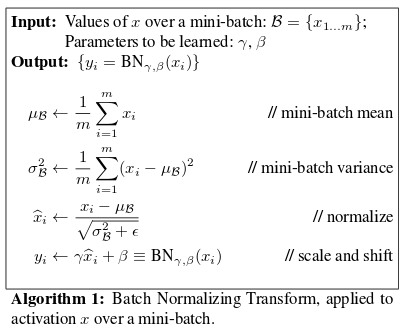
\includegraphics[scale=0.6]{imgs/batch_norm.PNG}
\vskip 0.1in

Steps are the following:
\begin{enumerate}
\item Calculate the batch mean of the values $x$ of a particular layer (that we do the normalization on) $\mu_{\beta}$
\item Similarly, calculate the variance of those values $x$ for this layer $\sigma_{\beta}^{2}$
\item Normalize the values, substracting the mean $\mu_{\beta}$ and dividing by STD (+constant) $\sqrt{\sigma_{\beta}^{2} + \epsilon}$. This will result in a new Gaussian distribution with mean of 0 and Variance of 1. 
\item Scale and Shift by learnable parameters $\gamma$ and $\beta$. Those parameters are being learned, and are inserted to make it possible to the distribution to be scaled and shifted if such is needed. For example, if it is of our interest to make the batch normalization an identity transform. 
\end{enumerate}

\newpage



\end{document}



















